\chapter{Optical Detection}

Detecting light and converting it into a measurable signal is the basis of most experimental observations in physics, from astronomy and spectroscopy to metrology and medicine. For centuries the only detectors were the human eye and, since the nineteenth century, photographic plates, which store an image but do not provide a quantitative electrical output. The explanation of the photoelectric effect by Einstein in 1905 opened the way to detectors that convert photons into electrons: vacuum phototubes and photomultiplier tubes in the first half of the twentieth century, and later semiconductor photodiodes, which are compact, fast and inexpensive. The development of CMOS image sensors integrated the pixels with readout electronics, making digital cameras small, cheap and ubiquitous \cite{stefanovCMOSImageSensors2023}.

In the context of interferometry, the detector is the element that turns the fringe pattern into data, and the problem addressed in this work is to measure distances precisely both in space and in time. In space, the pattern has a period of the order of millimeters, and recovering the position of the fringes and the direction of their motion requires an array of pixels able to resolve it. Every time the mirror moves by half a wavelength one fringe goes by, so the fringe rate grows linearly with the mirror velocity and the detector must sample fast enough not to lose any fringe. These two requirements pull in opposite directions: a pixel array provides spatial information but is limited by its frame rate, whereas a single photodiode has a wide bandwidth but carries no spatial information.

The approach proposed in this work is to use both types of detector, each one for what it does best. A low-cost USB webcam, the Logitech C270, provides the spatial information of the pattern, including the direction of the fringe movement and the possibility of interpolating between fringes to reach a finer spatial resolution. A photodiode provides a high speed response, thus enabling high temporal resolution at the cost of lower spatial resolution.

This chapter presents the camera and its acquisition interface, the photodiode with its conditioning circuit, and the limits that the sampling rate imposes on the measurable velocity and the precision of each detector, closing with a validation of the digital acquisition chain using a pulsed LED.

\section{Camera}
\label{sec:c270}

The camera used in this project is the C270 HD WEBCAM, shown in \cref{fig:camera}, a USB 2.0 webcam manufactured by Logitech. It features a CMOS sensor capable of capturing video at a resolution of 640 x 480 pixels at 30 frames per second. Its compact design and USB interface allow for easy integration into the experimental setup for real-time image acquisition and processing of the interferometer fringes pattern.

This camera was selected due to its balance between cost and performance, while it may not offer high speed or high-resolution capabilities, it is sufficient for the requirements of this project in a calibration stage. The camera's output is processed by a common python library used for computer vision tasks, OpenCV.

\begin{figure}[htbp]
    \centering
    \begin{subfigure}{0.45\textwidth}
        \centering
        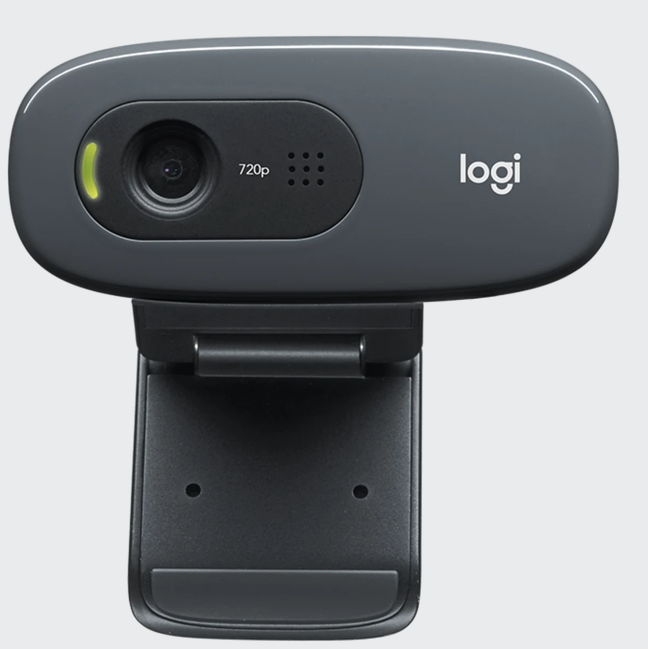
\includegraphics[width=\textwidth]{images/camera.png}
        \caption{C270 HD WEBCAM}
        \label{fig:camera}
    \end{subfigure}\hfill
    \begin{subfigure}{0.45\textwidth}
        \centering
        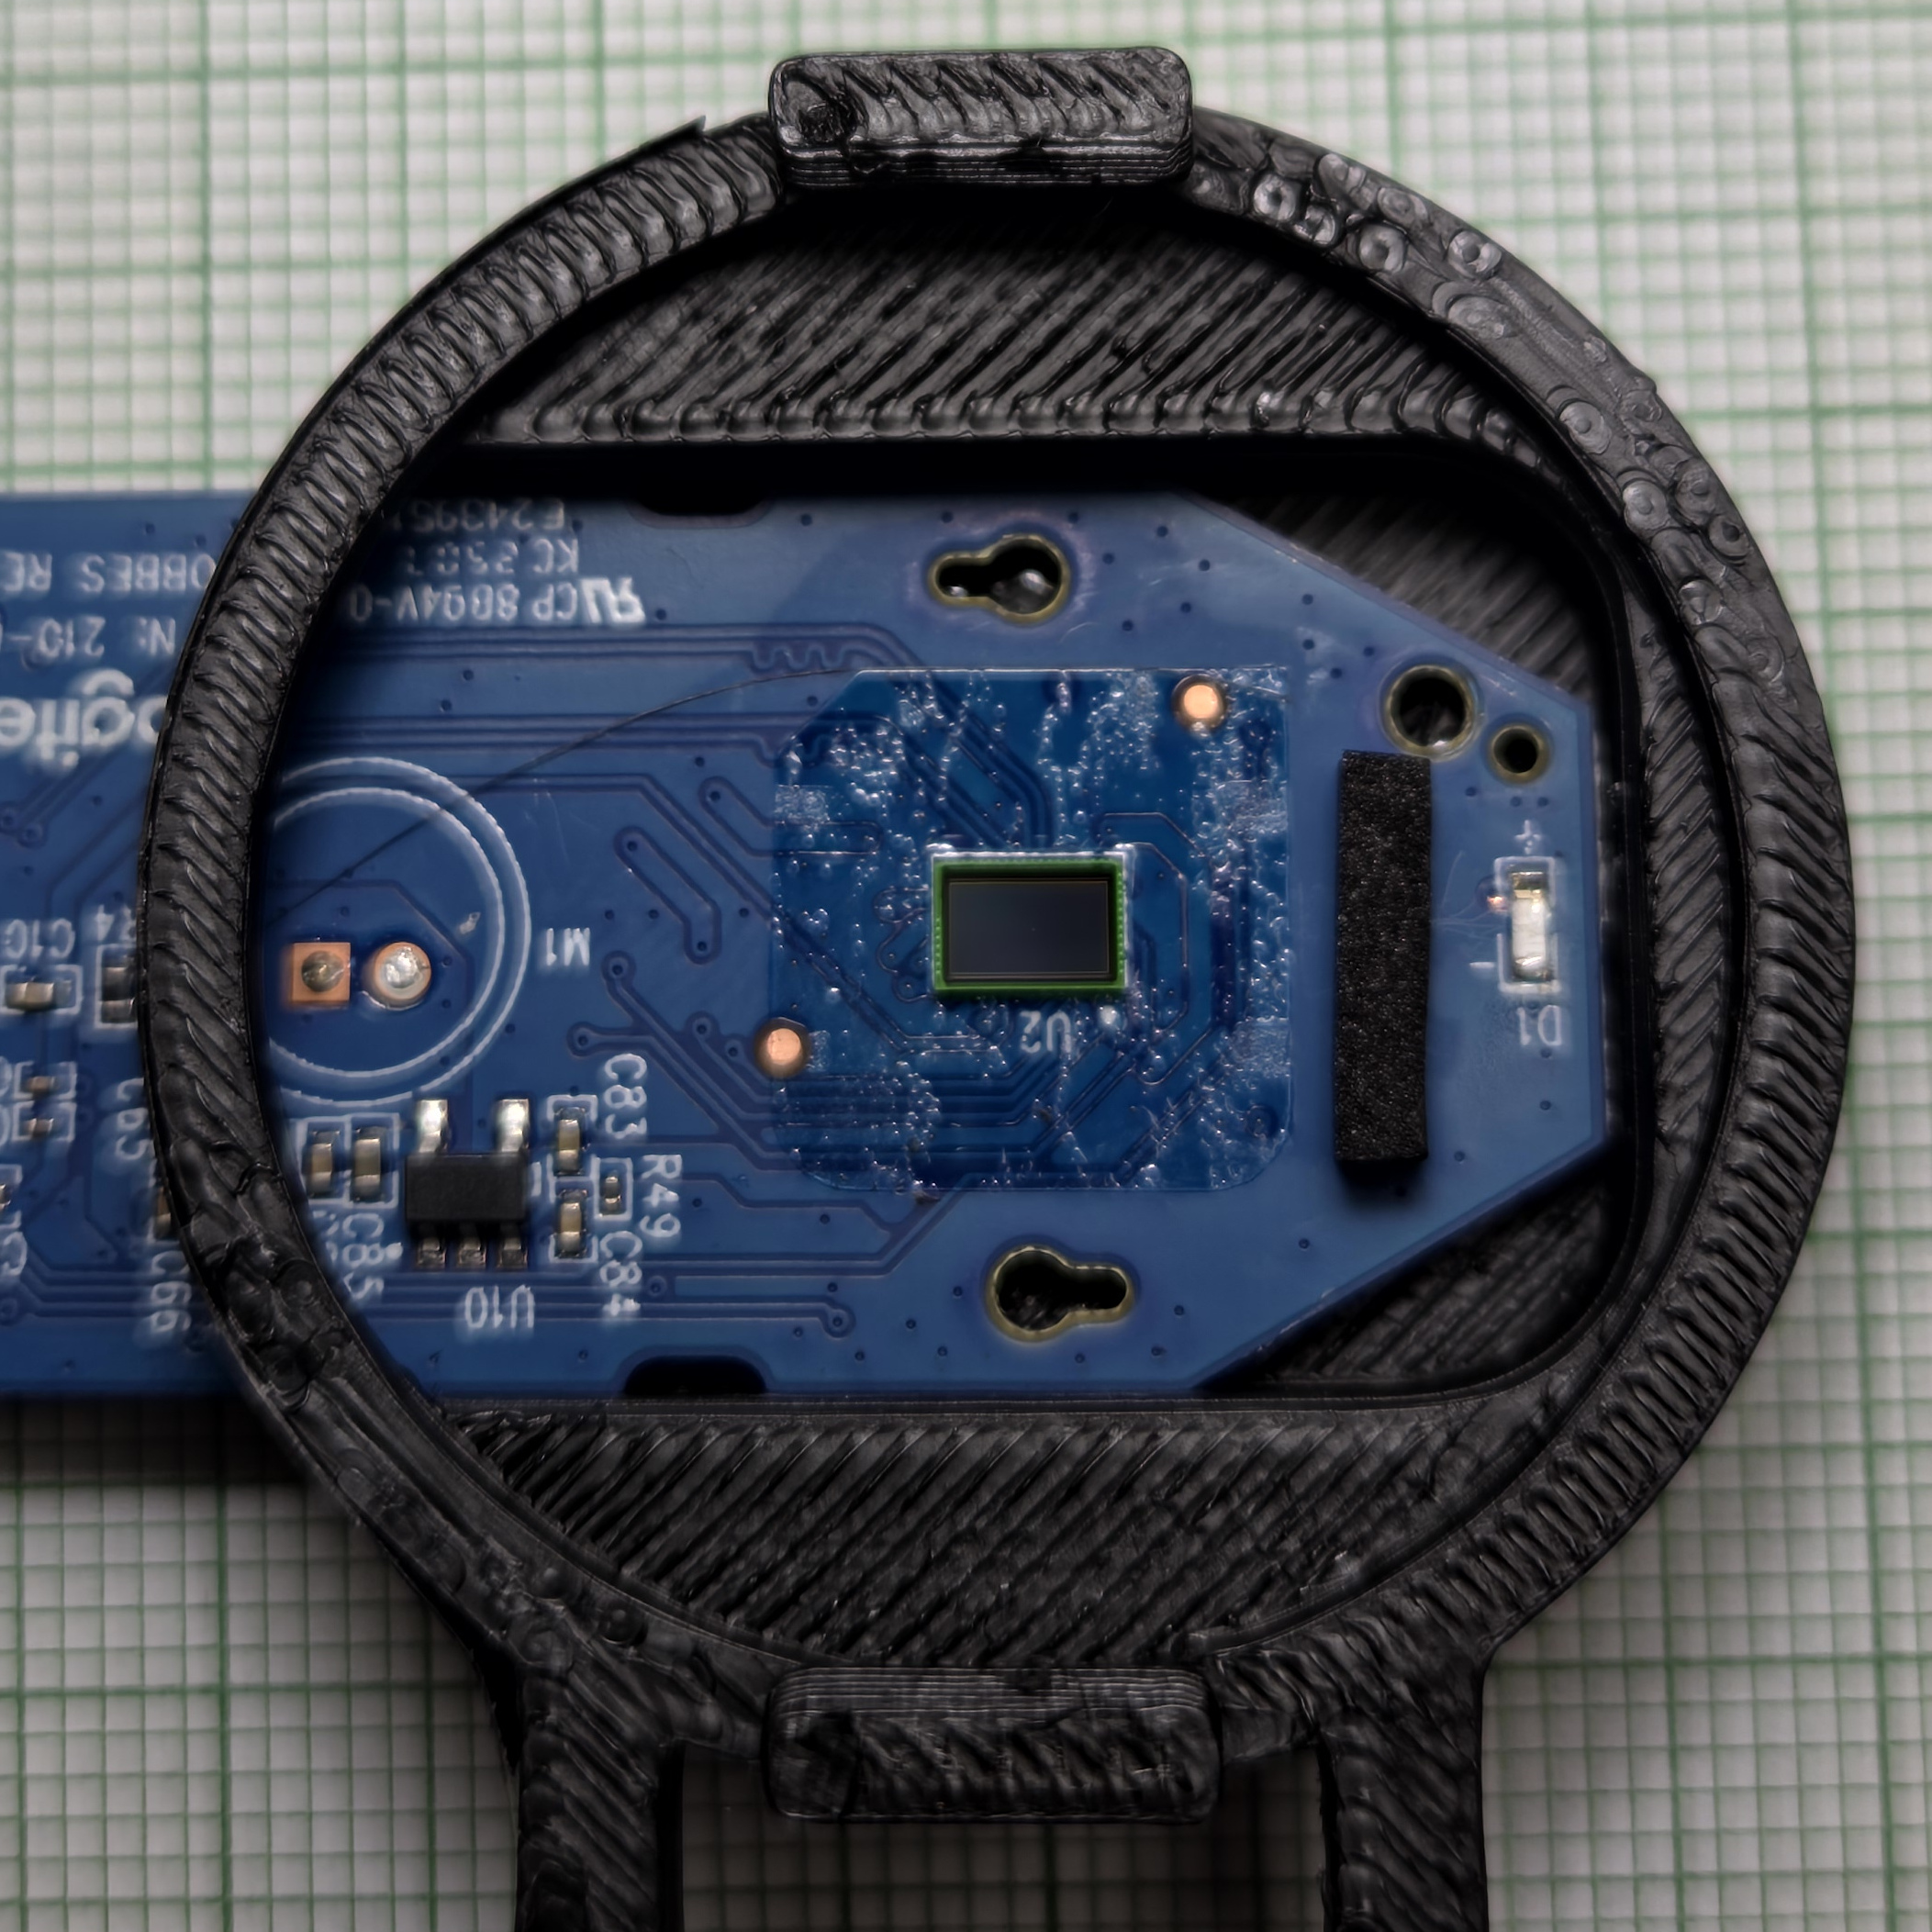
\includegraphics[width=\textwidth]{images/c270_on_holder.jpg}
        \caption{Camera Sensor with 3D Printed Support}
        \label{fig:camera_exposed}
    \end{subfigure}
    \caption{Camera Experimental Setup. a) C270 HD WEBCAM; b) Camera Sensor with 3D Printed Support for coupling to the interferometer setup.}
    \label{fig:camera_setup}
\end{figure}

The camera is dismantled to access the sensor directly, allowing for a more compact and flexible integration into the experimental setup, the lens was removed to avoid distortion of the pattern \cref{fig:camera_exposed}. A 3d printed support was designed to hold the camera in place, ensuring stability and proper alignment with the interferometer's optical path. The camera is connected to a computer via USB, where the acquired images are processed in real-time to extract the fringes and count their movement. This support belongs to a modular set of 3D-printed mounts, described in \cref{sec:experimental_setup}.


\subsection{Acquisition Graphical User Interface}
\label{sec:camera_gui}

To apply the ROI-based fringe tracking described in \cref{sec:roi_fringe_velocity} to the frames delivered by the C270 camera (\cref{sec:c270}), a custom graphical user interface (GUI) was developed. It gathers in a single window the live camera view, the placement and adjustment of the $\text{ROI}$, the real-time plot of the mean ROI irradiance, and the control of the stepper motor that drives the movable mirror, so that an experiment can be configured, executed and monitored without leaving the application. The interface is shown in \cref{fig:camera_ui}.

\begin{figure}[htbp]
    \centering
    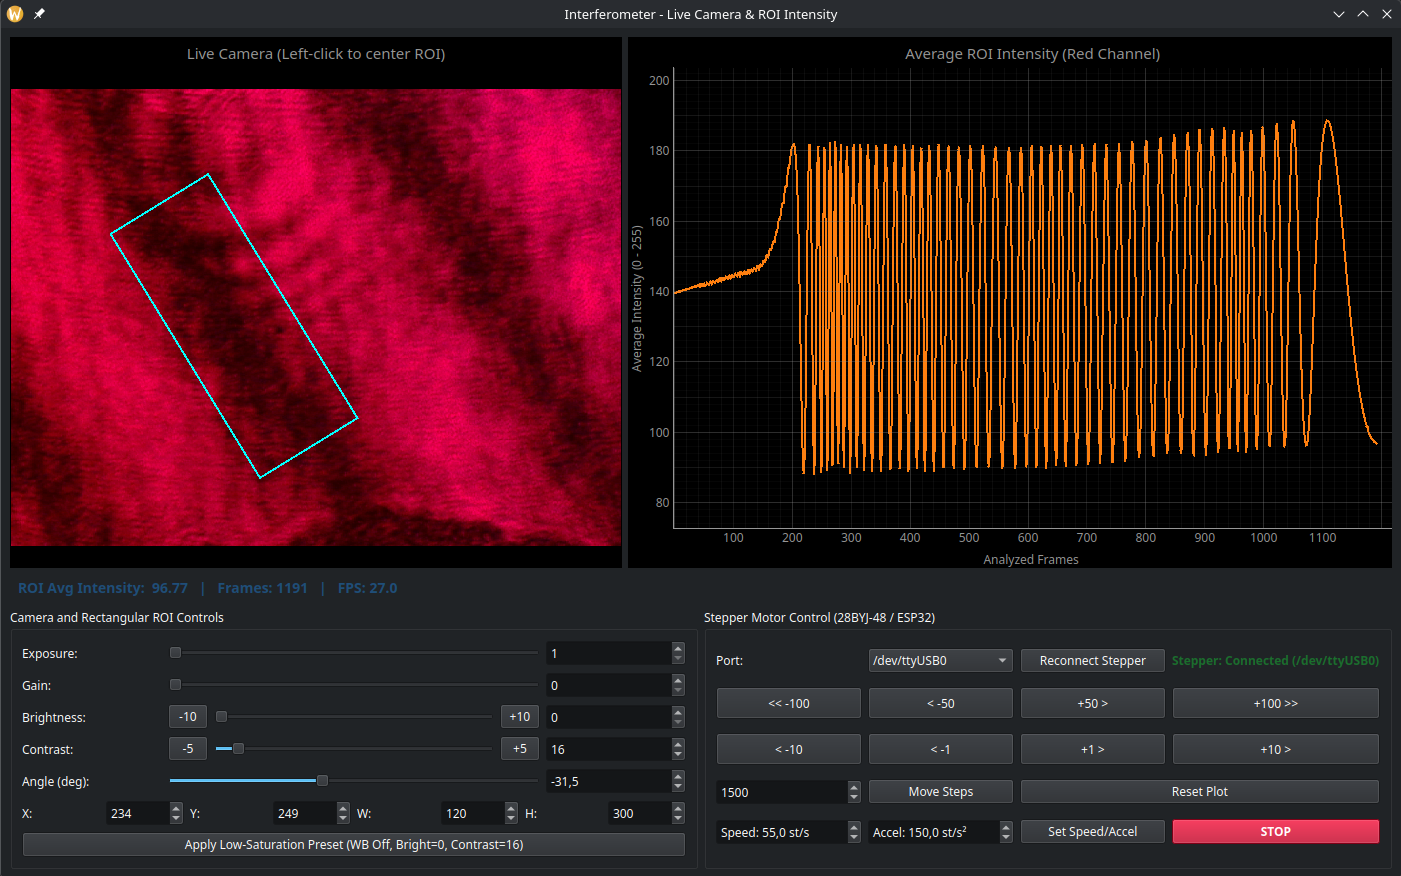
\includegraphics[width=\textwidth]{images/camera_ui.png}
    \caption{Graphical user interface for live fringe acquisition. Top left: live camera view with the rotated rectangular $\text{ROI}$ (cyan); top right: average $\text{ROI}$ intensity of the red channel versus analyzed frames; middle: status line with ROI average intensity, frame counter and FPS; bottom left: camera and $\text{ROI}$ controls; bottom right: stepper motor control.}
    \label{fig:camera_ui}
\end{figure}

The window is divided into the following regions:
\begin{itemize}
    \item \textbf{Live camera view:} Displays the frames captured by the camera in real time. The $\text{ROI}$ is drawn over the image as a cyan rectangle and can be re-centered at any moment with a left click on the desired position. The $\text{ROI}$ can be rotated by an angle (in degrees), allowing its long side to be aligned with the local fringe direction and its width $W$ to be matched to the fringe period $\Lambda_x$, which controls the attenuation of the modulation amplitude in \cref{eq:roi_sinc_attenuation}.

    \item \textbf{ROI intensity plot:} For every analyzed frame $k$, the mean irradiance $\bar{I}_{\text{ROI}}(t_k)$ of the red channel inside the $\text{ROI}$ \cref{eq:roi_mean_irradiance} is appended to a live plot, with intensity in the $0$--$255$ range on the vertical axis and the number of analyzed frames on the horizontal axis. Each oscillation of the trace corresponds to a fringe crossing the $\text{ROI}$, so the maxima and minima used to count fringes and compute the mirror displacement \cref{eq:roi_step_displacement} can be inspected visually.

    \item \textbf{Status line:} Reports the current ROI average intensity, the number of frames processed and the effective frame rate (FPS). The latter is relevant because the maximum measurable velocity is limited by the sampling rate (see \cref{sec:camera_velocity}); in the example the camera runs at $27.0$ FPS, slightly below the nominal $30$ FPS.

    \item \textbf{Camera and ROI controls:} Sliders and numeric fields set the exposure, gain, brightness and contrast of the camera, together with the $\text{ROI}$ geometry ($X$, $Y$, $W$, $H$ and angle). A \emph{low-saturation preset} button disables the automatic white balance and sets brightness to $0$ and contrast to $16$. Avoiding pixel saturation is important because a clipped signal flattens the peaks of $\bar{I}_{\text{ROI}}(t_k)$ and degrades the detection of maxima and minima.

    \item \textbf{Stepper motor control:} Communicates over a serial port with the ESP32 that drives the 28BYJ-48 stepper motor. The panel allows selecting the port and reconnecting, moving a relative number of steps with the quick buttons ($\pm 1$, $\pm 10$, $\pm 50$, $\pm 100$) or an arbitrary count with \emph{Move Steps}, setting the cruise speed (steps/s) and acceleration (steps/s$^2$), clearing the plot with \emph{Reset Plot} before a new measurement, and stopping the motor immediately with the \emph{STOP} button.
\end{itemize}

During the Openflexure calibration, the operator positions and orients the $\text{ROI}$, applies the low-saturation preset, resets the plot and commands a known number of motor steps. The fringes counted in the resulting trace, together with \cref{eq:roi_step_displacement}, give the mirror displacement associated with that step count, from which the step size of the stage is obtained.

\subsection{Fringe Movement to Mirror Displacement and Velocity}
\label{sec:fringe_to_displacement_velocity}

A detector only delivers intensity values; to obtain a physical quantity such as a displacement or a velocity, those values must be linked to the quantity of interest through a model. In interferometry this link is the fringe count: since Michelson used it to express the meter in wavelengths of light, the passage of fringes has been the way of converting a change of optical path into a length. Establishing this relation is what turns the interferometer and its detectors from an instrument that produces a pattern into an instrument that measures.

For this work the theoretical background is relevant for several reasons. It fixes the displacement associated with each fringe, and     therefore the resolution that fringe counting can reach (\cref{eq:displacement_m2}). It relates the velocity of the mirror to the rate at which fringes cross the detector (\cref{eq:velocity_fringe_rate}), which is the quantity that limits how fast the mirror can move before the camera starts to lose fringes (\cref{sec:camera_velocity}). It also shows that a single intensity value cannot tell in which direction the mirror moves, since the sign of the motion is encoded in the direction of the fringe progression, which motivates the use of the camera and its spatial information.

The following sections derive the relation between fringe movement, mirror displacement and velocity, and then present the method used to apply it to the frames of the camera by tracking the irradiance of a region of interest (\cref{sec:roi_fringe_velocity}), together with the graphical interface that implements it (\cref{sec:camera_gui}).

Let $L_2(t)$ denote the optical path length from $\text{BS}$ to the movable mirror $M2$ at time $t$, and let $L_1$ denote the constant optical path length along the fixed path to $M1$. Because each beam traverses the distance between $\text{BS}$ and its corresponding mirror twice, the round-trip optical path difference in a medium of refractive index $n$ (with $n \approx 1$ in air) is
\begin{equation}
    \Delta(t) = 2n\bigl[L_2(t) - L_1\bigr] + \Delta_0
    \label{eq:opd_m2}
\end{equation}
where $\Delta_0$ accounts for any constant phase-shift offset (such as reflection phase differences at $\text{BS}$ and the mirrors).

\subsubsection{Mirror Displacement from Fringe Shift}
Suppose the shift of $\Delta m = 1$ corresponds to a mirror displacement of $\Delta d_{M2} = \lambda/2$ along the axis of beam $(2)$. Tracking continuous phase $\delta(t)$ rather than integer fringe counts alone also permits sub-fringe displacement measurement.

\subsubsection{Mirror Velocity from Fringe Shift}
Differentiating \cref{eq:displacement_m2} with respect to time yields the velocity $v_{M2}(t)$ of the movable mirror $M2$:
\begin{equation}
    v_{M2}(t) = \frac{\lambda}{2}\,\frac{dm(t)}{dt}
    \label{eq:velocity_m2}
\end{equation}

In terms of the fringe-crossing rate (temporal fringe frequency) $f_{\text{fringe}}(t) = \frac{dm(t)}{dt}$ observed at a fixed detector or camera ROI along output beam $(4)$, the mirror speed is
\begin{equation}
    v_{M2}(t) = \frac{\lambda}{2n}\,f_{\text{fringe}}(t)
    \label{eq:velocity_fringe_rate}
\end{equation}


Alternatively, if a spatial fringe feature shifts across a coordinate axis $x$ perpendicular to the fringe normal with spatial fringe period $\Lambda_x$ and fringe-shift speed $v_{\text{fringe}}(t) = \frac{dx(t)}{dt}$, then $f_{\text{fringe}}(t) = \frac{v_{\text{fringe}}(t)}{\Lambda_x}$, giving
\begin{equation}
    v_{M2}(t) = \frac{\lambda}{2n}\,\frac{v_{\text{fringe}}(t)}{\Lambda_x}
    \label{eq:velocity_spatial_shift}
\end{equation}


The sign of $\Delta d_{M2}$ and $v_{M2}(t)$ is determined by the direction of fringe progression, which corresponds to $M2$ moving toward or away from $\text{BS}$ along beam $(2)$. The movable mirror $M2$ translates along the optical axis of beam $(2)$ by a displacement $\Delta d_{M2} = d_{M2}(t_2) - d_{M2}(t_1)$ between two instants $t_1$ and $t_2$. This changes the round-trip optical path length by $2\,\Delta d_{M2}$, producing a corresponding change in the interference phase difference $\delta = \frac{2\pi}{\lambda}\Delta$:
\begin{equation}
    \Delta\delta = \frac{4\pi}{\lambda}\,\Delta d_{M2}
    \label{eq:phase_shift_m2}
\end{equation}

Where $\lambda$ is the wavelength of the laser source.


Because each full fringe cycle (from one bright maximum to the next, or one dark minimum to the next) corresponds to a phase change of $\Delta\delta = 2\pi\,\Delta m$, where $\Delta m$ is the net number of fringes passing a fixed observation point or region of interest (ROI), substituting into \cref{eq:phase_shift_m2} gives the axial displacement of mirror $M2$:
\begin{equation}
    \Delta d_{M2} = \frac{\lambda}{2}\,\Delta m
    \label{eq:displacement_m2}
\end{equation}


Each fringe shift of $\Delta m = 1$ corresponds to a mirror displacement of $\Delta d_{M2} = \lambda/2$ along the axis of beam $(2)$. Tracking continuous phase $\delta(t)$ rather than integer fringe counts alone also permits sub-fringe displacement measurement.
\subsection{ROI-Based Fringe Tracking and Velocity Estimation}
\label{sec:roi_fringe_velocity}

In the experimental acquisition pipeline, frames of resolution $640 \times 480\text{ pixels}$ are captured at a sampling rate of $f_s = 30\text{ frames per second}$ (frame period $T_s = \frac{1}{f_s} \approx 33.33\text{ ms}$) \cref{sec:c270}. Rather than processing the entire sensor frame, a localized region of interest ($\text{ROI}$) spanning approximately one full fringe width is placed over a high-contrast region of the fringe pattern to track temporal irradiance modulation and fringe progression as movable mirror $M2$ translates along beam $(2)$ axis \cref{fig:schematic_michelson_interferometer}.



\subsubsection{ROI Mean-Irradiance Model}
\label{sec:roi_model_validity}

Starting from the two-beam interference model with fringe visibility of \cref{eq:visibility_irradiance} (\cref{sec:two_beam_interference}), the irradiance averaged over a small $\text{ROI}$ can be modeled as follows.

When spatially averaging $I(x, y, t_k)$ over a localized rectangular $\text{ROI}$ of dimensions $W \times H$ centered at $(x_0, y_0)$, the phase field can be approximated to first order as $\delta(x, y, t_k) \approx \delta_0(t_k) + k_x(x - x_0) + k_y(y - y_0)$, where $\delta_0(t_k)$ is the temporal phase at the $\text{ROI}$ center and $k_x = 2\pi/\Lambda_x$, $k_y = 2\pi/\Lambda_y$ represent the local spatial fringe wavenumbers. Assuming $I_0'$ and $V$ vary slowly across the small window, integrating over the $\text{ROI}$ yields:
\begin{equation}
    \bar{I}_{\text{ROI}}(t_k) \approx I_{\text{bg}} + I_{\text{amp}}\cos\!\bigl(\delta_0(t_k)\bigr)
    \label{eq:roi_irradiance_model_justified}
\end{equation}
where $I_{\text{bg}} \approx I_0'$ and the effective modulation amplitude is attenuated by spatial averaging according to
\begin{equation}
    I_{\text{amp}} \approx I_0'\,V\,\operatorname{sinc}\!\left(\frac{W}{\Lambda_x}\right)\operatorname{sinc}\!\left(\frac{H}{\Lambda_y}\right), \qquad \operatorname{sinc}(u) = \frac{\sin(\pi u)}{\pi u}
    \label{eq:roi_sinc_attenuation}
\end{equation}

\subsubsection{ROI Mean Irradiance and Classification}

\begin{figure}[htbp]
    \centering
    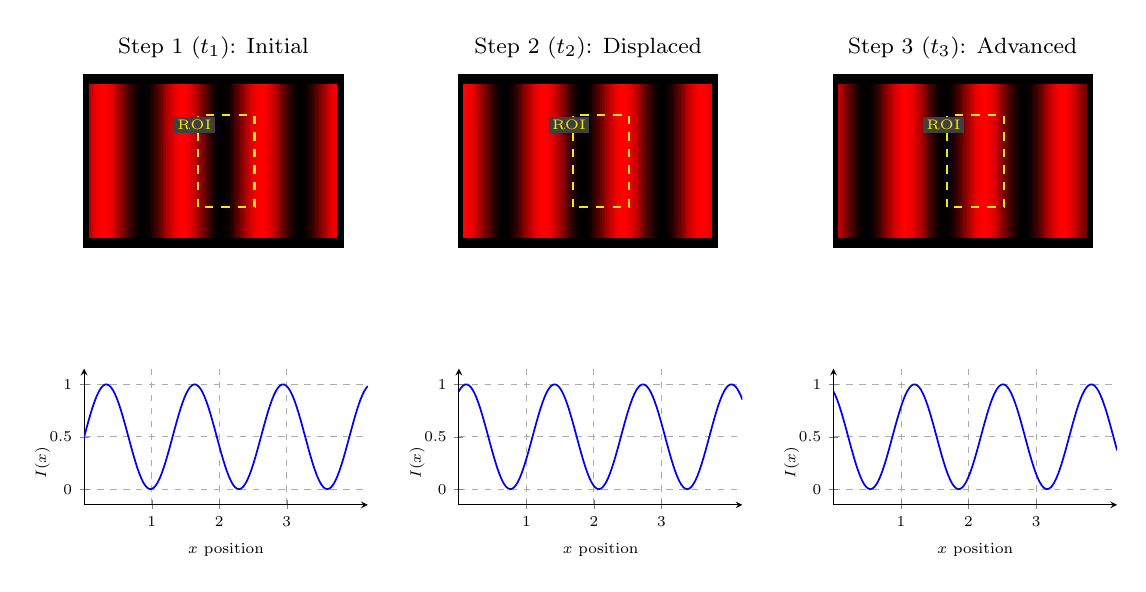
\begin{tikzpicture}[scale=0.78]
        % ==========================================
        % STEP 1: t_1 (Initial Position)
        % ==========================================
        \begin{scope}[shift={(0,0)}]
            % Camera View Box
            \draw[thick, fill=black] (0,4.2) rectangle (4.2,7.0);
            \node[above, font=\footnotesize] at (2.1,7.1) {Step 1 ($t_1$): Initial};
            \foreach \x in {0.10, 0.13, ..., 4.10} {
                \pgfmathsetmacro{\irradiance}{sin(\x * 280)*50 + 50}
                \draw[color=red!\irradiance!black, line width=0.45mm] (\x, 4.35) -- (\x, 6.85);
            }
            % ROI highlight box (~1 fringe wide: width = 1.35)
            \draw[dashed, yellow!95!black, thick] (1.85, 4.85) rectangle (2.77, 6.35);
            \node[fill=black!75, text=yellow!95!black, inner sep=1.2pt, font=\tiny, anchor=north west] at (1.45, 6.32) {ROI};
            \draw[thick] (0,4.2) rectangle (4.2,7.0);

            % Enlarged irradiance Plot
            \begin{axis}[
                at={(-0.4,0)},
                anchor=south west,
                width=6.2cm,
                height=3.8cm,
                xmin=0, xmax=4.2,
                ymin=-0.15, ymax=1.15,
                axis lines=left,
                xlabel={$x$ position},
                ylabel={$I(x)$},
                font=\scriptsize,
                xtick={1, 2, 3},
                ytick={0, 0.5, 1},
                grid=major,
                grid style={dashed, gray!65},
                xlabel style={below=1pt},
                ylabel style={left=1pt}
            ]
                \addplot[domain=0:4.2, samples=140, thick, blue] {sin(deg(x*4.8))*0.5 + 0.5};
            \end{axis}
        \end{scope}

        % ==========================================
        % STEP 2: t_2 (Intermediate Displacement)
        % ==========================================
        \begin{scope}[shift={(6.1,0)}]
            % Camera View Box
            \draw[thick, fill=black] (0,4.2) rectangle (4.2,7.0);
            \node[above, font=\footnotesize] at (2.1,7.1) {Step 2 ($t_2$): Displaced};
            \foreach \x in {0.10, 0.13, ..., 4.10} {
                \pgfmathsetmacro{\irradiance}{sin(\x * 280 + 60)*50 + 50}
                \draw[color=red!\irradiance!black, line width=0.45mm] (\x, 4.35) -- (\x, 6.85);
            }
            % ROI highlight box (~1 fringe wide: width = 1.35)
            \draw[dashed, yellow!95!black, thick] (1.85, 4.85) rectangle (2.77, 6.35);
            \node[fill=black!75, text=yellow!95!black, inner sep=1.2pt, font=\tiny, anchor=north west] at (1.45, 6.32) {ROI};
            \draw[thick] (0,4.2) rectangle (4.2,7.0);

            % Enlarged irradiance Plot
            \begin{axis}[
                at={(-0.4,0)},
                anchor=south west,
                width=6.2cm,
                height=3.8cm,
                xmin=0, xmax=4.2,
                ymin=-0.15, ymax=1.15,
                axis lines=left,
                xlabel={$x$ position},
                ylabel={$I(x)$},
                font=\scriptsize,
                xtick={1, 2, 3},
                ytick={0, 0.5, 1},
                grid=major,
                grid style={dashed, gray!65},
                xlabel style={below=1pt},
                ylabel style={left=1pt}
            ]
                \addplot[domain=0:4.2, samples=140, thick, blue] {sin(deg(x*4.8) + 60)*0.5 + 0.5};
            \end{axis}
        \end{scope}

        % ==========================================
        % STEP 3: t_3 (Advanced Displacement)
        % ==========================================
        \begin{scope}[shift={(12.2,0)}]
            % Camera View Box
            \draw[thick, fill=black] (0,4.2) rectangle (4.2,7.0);
            \node[above, font=\footnotesize] at (2.1,7.1) {Step 3 ($t_3$): Advanced};
            \foreach \x in {0.10, 0.13, ..., 4.10} {
                \pgfmathsetmacro{\irradiance}{sin(\x * 280 + 120)*50 + 50}
                \draw[color=red!\irradiance!black, line width=0.45mm] (\x, 4.35) -- (\x, 6.85);
            }
            % ROI highlight box (~1 fringe wide: width = 1.35)
            \draw[dashed, yellow!95!black, thick] (1.85, 4.85) rectangle (2.77, 6.35);
            \node[fill=black!75, text=yellow!95!black, inner sep=1.2pt, font=\tiny, anchor=north west] at (1.45, 6.32) {ROI};
            \draw[thick] (0,4.2) rectangle (4.2,7.0);

            % Enlarged irradiance Plot
            \begin{axis}[
                at={(-0.4,0)},
                anchor=south west,
                width=6.2cm,
                height=3.8cm,
                xmin=0, xmax=4.2,
                ymin=-0.15, ymax=1.15,
                axis lines=left,
                xlabel={$x$ position},
                ylabel={$I(x)$},
                font=\scriptsize,
                xtick={1, 2, 3},
                ytick={0, 0.5, 1},
                grid=major,
                grid style={dashed, gray!65},
                xlabel style={below=1pt},
                ylabel style={left=1pt}
            ]
                \addplot[domain=0:4.2, samples=140, thick, blue] {sin(deg(x*4.8) + 120)*0.5 + 0.5};
            \end{axis}
        \end{scope}
    \end{tikzpicture}
    \caption{Sequential time-steps ($t_1, t_2, t_3$) showing the fringe field, a single-fringe-width $\text{ROI}$ window, and 1D irradiance profiles $I(x)$ as movable mirror $M2$ translates.}
    \label{fig:three_step_fringes}
\end{figure}


For discrete frame index $k = 0, 1, 2, \dots$ acquired at time $t_k = k T_s = \frac{k}{f_s}$, let $I(x, y, t_k)$ denote the pixel irradiance within the $\text{ROI}$ (comprising $N_{\text{ROI}}$ pixels). The spatial mean irradiance inside the $\text{ROI}$ at frame $k$ is
\begin{equation}
    \bar{I}_{\text{ROI}}(t_k) = \frac{1}{N_{\text{ROI}}} \sum_{(x, y) \in \text{ROI}} I(x, y, t_k)
    \label{eq:roi_mean_irradiance}
\end{equation}

Neglecting slow variations, $\bar{I}_{\text{ROI}}(t_k)$ oscillates quasi-periodically with the interference phase difference $\delta(t_k)$:
\begin{equation}
    \bar{I}_{\text{ROI}}(t_k) \approx I_{\text{bg}} + I_{\text{amp}} \cos\!\bigl(\delta(t_k)\bigr)
    \label{eq:roi_irradiance_model}
\end{equation}
where $I_{\text{bg}}$ is the mean background level and $I_{\text{amp}}$ is the effective fringe modulation amplitude within the $\text{ROI}$. Using running or window extrema $\bar{I}_{\max}$ and $\bar{I}_{\min}$ estimated from recent frames, the normalized ROI irradiance is
\begin{equation}
    \tilde{I}_{\text{ROI}}(t_k) = \frac{\bar{I}_{\text{ROI}}(t_k) - \bar{I}_{\min}}{\bar{I}_{\max} - \bar{I}_{\min}} \in [0, 1]
    \label{eq:normalized_roi_irradiance}
\end{equation}

Maxima (constructive fringe peaks passing across the $\text{ROI}$) and minima (destructive dark fringes passing across the $\text{ROI}$) are identified from $\bar{I}_{\text{ROI}}(t_k)$ and its discrete temporal difference $\Delta \bar{I}_k = \bar{I}_{\text{ROI}}(t_k) - \bar{I}_{\text{ROI}}(t_{k-1})$:
\begin{itemize}
    \item \textbf{Local Maximum (Bright Fringe Center in ROI):} $\bar{I}_{\text{ROI}}(t_k)$ reaches a peak (or $\tilde{I}_{\text{ROI}}(t_k) \to 1$) where $\Delta \bar{I}_k$ transitions from positive to non-positive, corresponding to $\delta = 2\pi m$
    \item \textbf{Local Minimum (Dark Fringe Center in ROI):} $\bar{I}_{\text{ROI}}(t_k)$ reaches a trough (or $\tilde{I}_{\text{ROI}}(t_k) \to 0$) where $\Delta \bar{I}_k$ transitions from negative to non-negative, corresponding to $\delta = (2m + 1) \pi$
\end{itemize}
Because a single irradiance value cannot distinguish the rising slope ($\frac{d\bar{I}}{dt} > 0$) from the falling slope ($\frac{d\bar{I}}{dt} < 0$) at intermediate brightness levels, inspecting prior frames $t_{k-1}, t_{k-2}, \dots$ is necessary to resolve phase evolution and determine direction of movement, an schematic of this behavior is shown in \cref{fig:three_step_fringes}.

\subsubsection{Determining Direction from Frame History}
By combining the temporal history of $\bar{I}_{\text{ROI}}$ with local spatial/feature displacement across consecutive frames:
\begin{enumerate}
    \item \textbf{Slope and Extremum Sequence:} Comparing $\bar{I}_{\text{ROI}}(t_k)$ against $\bar{I}_{\text{ROI}}(t_{k-1})$ and $\bar{I}_{\text{ROI}}(t_{k-2})$ establishes whether the $\text{ROI}$ is currently traversing a rising half-cycle or falling half-cycle between consecutive maxima and minima.
    \item \textbf{Spatial Fringe Progression Across Frames:} Tracking a local fringe feature (or cross-correlating a 1D irradiance profile across the $\text{ROI}$ between frames $t_{k-1}$ and $t_k$) yields the signed spatial shift $\Delta x_{\text{fringe}, k}$ along the local fringe normal.
\end{enumerate}
Let $s_k \in \{+1, -1\}$ denote the signed direction indicator determined from frame history.

\subsubsection{Displacement and Velocity Equations}
Each complete fringe cycle ($\Delta m = 1$, from one maximum to the next or one minimum to the next) corresponds to a round-trip optical path change of $\lambda$, which equals an axial displacement of mirror $M2$ given by
\begin{equation}
    \Delta d_{M2, k} = s_k\,\frac{\lambda}{2}\,\Delta m_k
    \label{eq:roi_step_displacement}
\end{equation}
where $\Delta m_k$ is the fractional or integer fringe count accumulated between frame $k-1$ and frame $k$ (for instance, $\Delta m_k = 0.5$ between an adjacent maximum and minimum).

Over the frame interval $T_s = 1/f_s$, the mean axial velocity of mirror $M2$ during step $k$ is
\begin{equation}
    v_{M2, k} = \frac{\Delta d_{M2, k}}{T_s} = s_k\,\frac{\lambda}{2}\,f_s\,\Delta m_k = s_k\,\frac{\lambda}{2}\,f_{\text{fringe}, k}
    \label{eq:roi_step_velocity}
\end{equation}
where $f_{\text{fringe}, k} = f_s\,\Delta m_k$ is the instantaneous fringe-crossing frequency in $\text{Hz}$ (fringes per second).



\subsection{Acquisition Graphical User Interface (GUI)}
\label{sec:camera_gui}

To apply the ROI-based fringe tracking described in \cref{sec:roi_fringe_velocity} to the frames delivered by the C270 camera (\cref{sec:c270}), a custom graphical user interface (GUI) was developed. It gathers in a single window the live camera view, the placement and adjustment of the $\text{ROI}$, the real-time plot of the mean ROI irradiance, and the control of the stepper motor that drives the movable mirror, so that an experiment can be configured, executed and monitored without leaving the application. The interface is shown in \cref{fig:camera_ui}.

\begin{figure}[htbp]
    \centering
    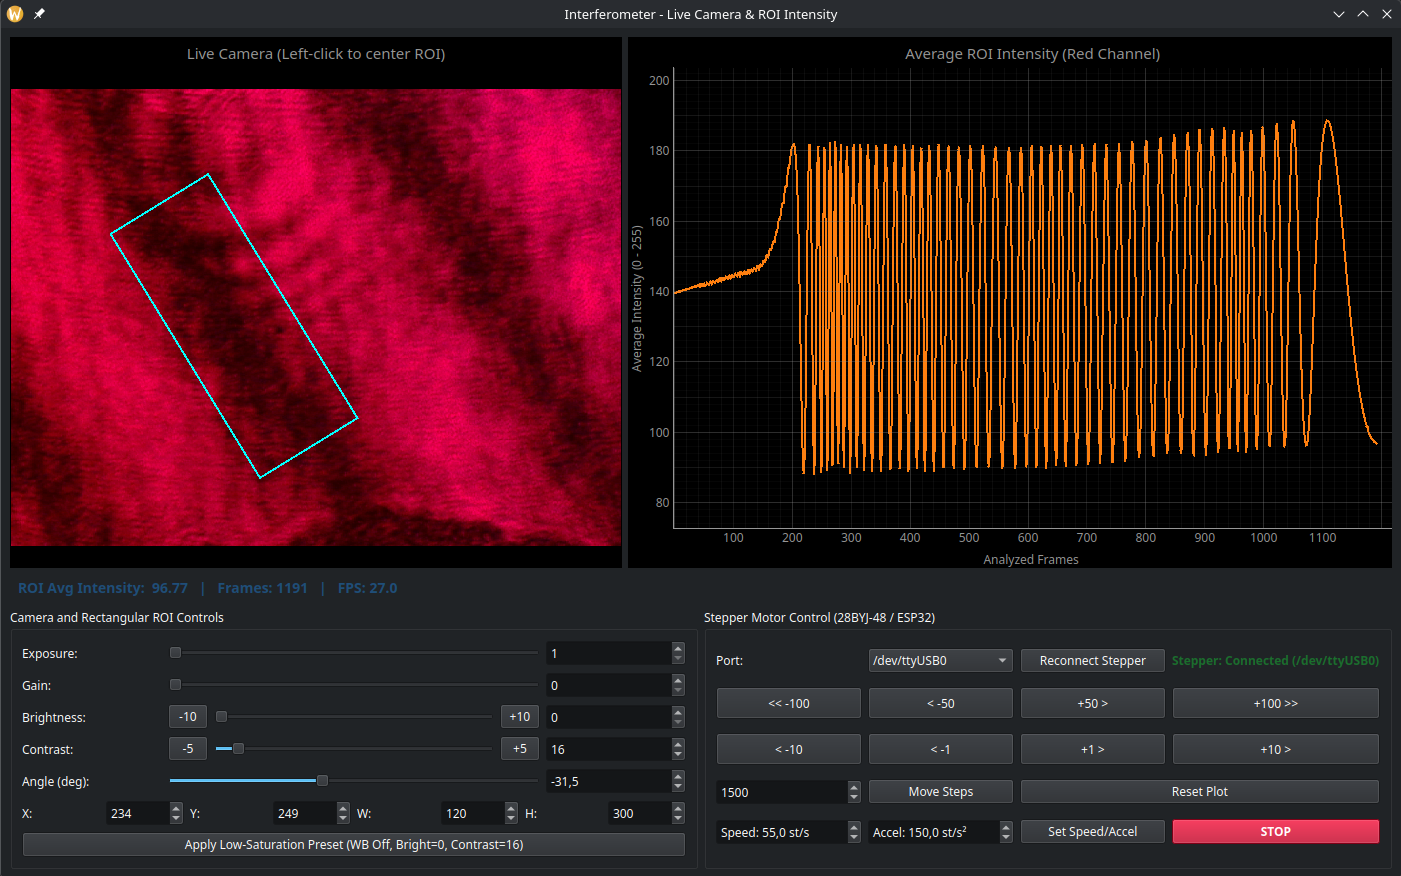
\includegraphics[width=\textwidth]{images/camera_ui.png}
    \caption{Graphical user interface for live fringe acquisition. Top left: live camera view with the rotated rectangular $\text{ROI}$ (cyan); top right: average $\text{ROI}$ intensity of the red channel versus analyzed frames; middle: status line with ROI average intensity, frame counter and FPS; bottom left: camera and $\text{ROI}$ controls; bottom right: stepper motor control.}
    \label{fig:camera_ui}
\end{figure}

The window is divided into the following regions:
\begin{itemize}
    \item \textbf{Live camera view:} Displays the frames captured by the camera in real time. The $\text{ROI}$ is drawn over the image as a cyan rectangle and can be re-centered at any moment with a left click on the desired position. The $\text{ROI}$ can be rotated by an angle (in degrees), allowing its long side to be aligned with the local fringe direction and its width $W$ to be matched to the fringe period $\Lambda_x$, which controls the attenuation of the modulation amplitude in \cref{eq:roi_sinc_attenuation}.

    \item \textbf{ROI intensity plot:} For every analyzed frame $k$, the mean irradiance $\bar{I}_{\text{ROI}}(t_k)$ of the red channel inside the $\text{ROI}$ \cref{eq:roi_mean_irradiance} is appended to a live plot, with intensity in the $0$--$255$ range on the vertical axis and the number of analyzed frames on the horizontal axis. Each oscillation of the trace corresponds to a fringe crossing the $\text{ROI}$, so the maxima and minima used to count fringes and compute the mirror displacement \cref{eq:roi_step_displacement} can be inspected visually.

    \item \textbf{Status line:} Reports the current ROI average intensity, the number of frames processed and the effective frame rate (FPS). The latter is relevant because the maximum measurable velocity is limited by the sampling rate (see \cref{sec:camera_velocity}); in the example the camera runs at $27.0$ FPS, slightly below the nominal $30$ FPS.

    \item \textbf{Camera and ROI controls:} Sliders and numeric fields set the exposure, gain, brightness and contrast of the camera, together with the $\text{ROI}$ geometry ($X$, $Y$, $W$, $H$ and angle). A \emph{low-saturation preset} button disables the automatic white balance and sets brightness to $0$ and contrast to $16$. Avoiding pixel saturation is important because a clipped signal flattens the peaks of $\bar{I}_{\text{ROI}}(t_k)$ and degrades the detection of maxima and minima.

    \item \textbf{Stepper motor control:} Communicates over a serial port with the ESP32 that drives the 28BYJ-48 stepper motor. The panel allows selecting the port and reconnecting, moving a relative number of steps with the quick buttons ($\pm 1$, $\pm 10$, $\pm 50$, $\pm 100$) or an arbitrary count with \emph{Move Steps}, setting the cruise speed (steps/s) and acceleration (steps/s$^2$), clearing the plot with \emph{Reset Plot} before a new measurement, and stopping the motor immediately with the \emph{STOP} button.
\end{itemize}

During the Openflexure movement measurement (see \cref{sec:experimental_setup}), the operator positions and orients the $\text{ROI}$, applies the low-saturation preset, resets the plot and commands a known number of motor steps. The fringes counted in the resulting trace, together with \cref{eq:roi_step_displacement}, give the mirror displacement associated with that step count, from which the step size of the stage is obtained.

\subsubsection{Conclusions}
\section{Photodiode}

Solid state detectors like the photodiode are based on the properties of semiconductors. These types of detectors have marked advantages over other types of detectors, they can be kept smaller than gas-filled detectors due to their density and also have better energy resolution than the scintillator counters \cite[Chap 11.]{knollRadiationDetectionMeasurement2010}. In this section, we will discuss the basic concepts of semiconductors and how they can be used as detectors.

\subsection{Semiconductors}
\subsubsection{Band Structure and Charge Carriers}

In crystalline solid materials, the periodic lattice structures restrict electron energies to distinct allowed bands that are separated by forbidden energies as shown in the diagram \cref{fig:band_structure}. The lower of these energy regions, known as the valence band, contains outer-shell electrons that are placed in a specific position inside the lattice via interatomic bonds. Conversely, the higher-lying conduction band represents free electrons capable of migrating through the crystal lattice and this electrons allow  electrical conductivity to be present. The magnitude of the forbidden energy gap or bandgap between these two bands dictates whether a material functions as an insulator or a semiconductor. 

In the absence of thermal excitation, both insulators and semiconductors maintain a completely filled valence band and a completely empty conduction band, resulting in no electrical conductivity under these baseline conditions. In contrast, metals feature not entirely filled highest energy band, permitting electrons to easily migrate within the crystal lattice with minimal incremental energy and thus ensuring high electrical conductivity across the material. For insulators and semiconductors, however, electrons must first cross the intervening bandgap to reach the conduction band, causing their baseline electrical conductivity to be many orders of magnitude lower \cite[Chap 11.]{knollRadiationDetectionMeasurement2010}.

\begin{figure}[htbp]
    \centering
    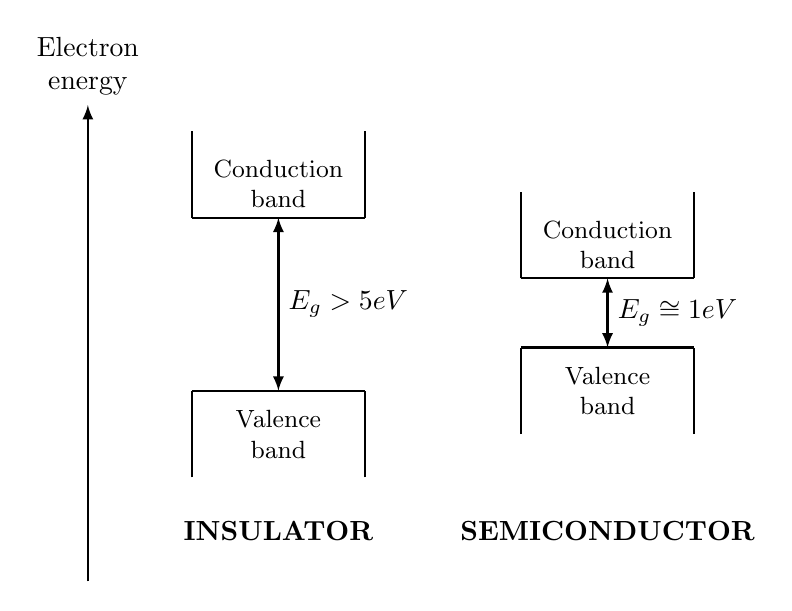
\begin{tikzpicture}[scale=1.1, >=latex]
        % Eje de energía vertical
        \draw[->, thick] (0,0) -- (0,5.5) node[above, align=center] {Electron\\energy};

        % --- AISLANTE (INSULATOR) ---
        \begin{scope}[shift={(1.2,0)}]
            % Banda de conducción
            \draw[thick] (0,4.2) -- (2.0,4.2);
            \node[above, align=center, font=\small] at (1.0,4.2) {Conduction\\band};
            \draw[thick] (0,4.2) -- (0,5.2);
            \draw[thick] (2.0,4.2) -- (2.0,5.2);

            % Flecha de banda prohibida (Eg > 5 eV)
            \draw[<->, thick] (1.0,2.2) -- node[right, align=left] {$E_g > 5\text{ eV}$} (1.0,4.2);

            % Banda de valencia
            \draw[thick] (0,2.2) -- (2.0,2.2);
            \draw[thick] (0,1.2) -- (0,2.2);
            \draw[thick] (2.0,1.2) -- (2.0,2.2);
            \node[align=center, font=\small] at (1.0, 1.7) {Valence\\band};

            % Etiqueta inferior
            \node[below, font=\bfseries] at (1.0, 0.8) {INSULATOR};
        \end{scope}

        % --- SEMICONDUCTOR ---
        \begin{scope}[shift={(5.0,0)}]
            % Banda de conducción
            \draw[thick] (0,3.5) -- (2.0,3.5);
            \node[above, align=center, font=\small] at (1.0,3.5) {Conduction\\band};
            \draw[thick] (0,3.5) -- (0,4.5);
            \draw[thick] (2.0,3.5) -- (2.0,4.5);

            % Flecha de banda prohibida (Eg ≈ 1 eV)
            \draw[<->, thick] (1.0,2.7) -- node[right, align=left] {$E_g \cong 1\text{ eV}$} (1.0,3.5);

            % Banda de valencia
            \draw[thick] (0,2.7) -- (2.0,2.7);
            \draw[thick] (0,1.7) -- (0,2.7);
            \draw[thick] (2.0,1.7) -- (2.0,2.7);
            \node[align=center, font=\small] at (1.0, 2.2) {Valence\\band};

            % Etiqueta inferior
            \node[below, font=\bfseries] at (1.0, 0.8) {SEMICONDUCTOR};
        \end{scope}

    \end{tikzpicture}
    \caption{Band structure for electron energies in insulators and semiconductors \cite[Chap 11.]{knollRadiationDetectionMeasurement2010}.}
    \label{fig:band_structure}
\end{figure}

At any temperature greater than zero the thermal energy introduced into the electrons within the lattice allows them to gain sufficient energy to cross the bandgap into the conduction band, leaving behind a vacancy known as a hole. This combination forms an electron-hole pair. Under the influence of an applied electric field, conduction electrons migrate toward positive potentials while positive holes move in the opposite direction, with the motion of both charge carriers contributing directly to the material's observed electrical conductivity. 

\begin{equation}
    p(T) = C T^{3/2} \exp\left(-\frac{E_g}{2kT}\right)
    \label{eq:thermal_generation}
\end{equation}

where:
\begin{itemize}
    \item $T =$ absolute temperature
    \item $E_g =$ bandgap energy
    \item $k =$ Boltzmann constant
    \item $C =$ proportionality constant characteristic of the material
\end{itemize}

The probability per unit time for thermal electron-hole pair generation is given by \cref{eq:thermal_generation} in \cite[p. 367]{knollRadiationDetectionMeasurement2010}. This generation of electron-hole pairs is heavily dependent on the ratio of the bandgap energy to the absolute temperature of the material. Consequently, materials with bigger bandgaps experience minimal thermal excitation that could create conductivity and thus act as insulators, while materials with smaller bandgaps yield sufficient conductivity to be classified as semiconductors. When there is no electric field pulling them apart, the electrons and holes created by heat eventually find each other and recombine canceling each other out. They constantly form and recombine until they reach a stable balance, this balance depends heavily on heat. If the material is cooled down, there is less thermal energy available, causing the number of active electron-hole pairs to drop drastically.


\subsubsection{Effect of Impurities on Semiconductors}

An ideal semiconductor without any traces of other elements or impurities is called an intrinsic semiconductor. The conductivity is then only determined by the electrons and holes generated by thermal excitation. However, in practice it is almost impossible to have a pure semiconductor, and the presence of impurities can significantly alter the electrical properties of the material. The process of intentionally adding impurities to a semiconductor is known as doping, and it can create two types of extrinsic semiconductors: n-type and p-type.

\begin{figure}[htbp]
    \centering
    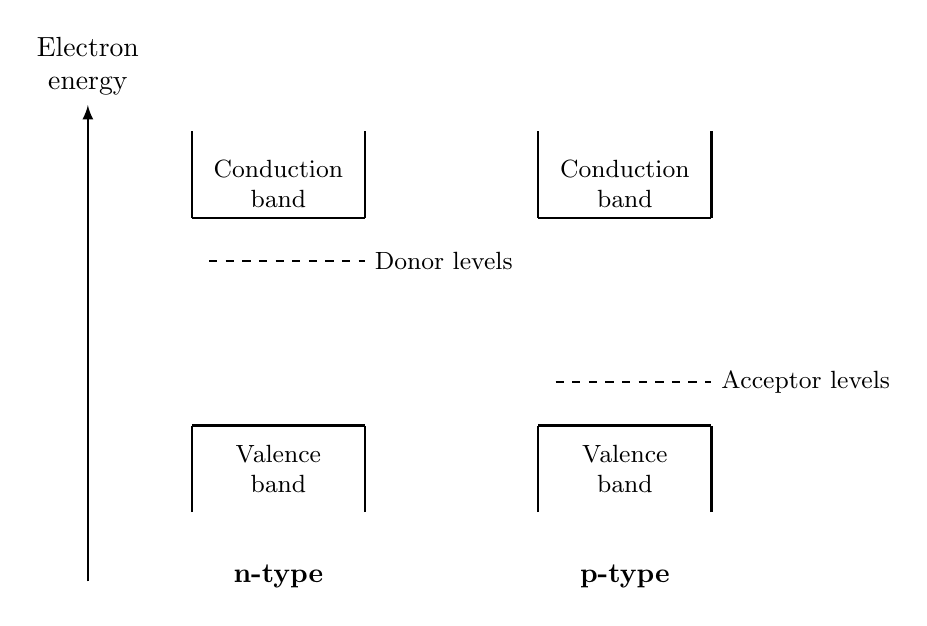
\begin{tikzpicture}[scale=1.1, >=latex]
        % Eje de energía vertical compartido
        \draw[->, thick] (0,0) -- (0,5.5) node[above, align=center] {Electron\\energy};

        % ==========================================
        % 1. N-TYPE SEMICONDUCTOR (Donor levels)
        % ==========================================
        \begin{scope}[shift={(1.2,0)}]
            % Banda de conducción
            \draw[thick] (0,4.2) -- (2.0,4.2);
            \node[above, align=center, font=\small] at (1.0,4.2) {Conduction\\band};
            \draw[thick] (0,4.2) -- (0,5.2);
            \draw[thick] (2.0,4.2) -- (2.0,5.2);

            % Niveles donantes (línea discontinua)
            \draw[thick, dashed] (0.2, 3.7) -- (2.0, 3.7);
            \node[right, font=\small] at (2.0, 3.7) {Donor levels};

            % Banda de valencia
            \draw[thick] (0,1.8) -- (2.0,1.8);
            \draw[thick] (0,0.8) -- (0,1.8);
            \draw[thick] (2.0,0.8) -- (2.0,1.8);
            \node[align=center, font=\small] at (1.0, 1.3) {Valence\\band};

            % Etiqueta inferior
            \node[below, font=\bfseries] at (1.0, 0.3) {n-type};
        \end{scope}

        % ==========================================
        % 2. P-TYPE SEMICONDUCTOR (Acceptor levels)
        % ==========================================
        \begin{scope}[shift={(5.2,0)}]
            % Banda de conducción
            \draw[thick] (0,4.2) -- (2.0,4.2);
            \node[above, align=center, font=\small] at (1.0,4.2) {Conduction\\band};
            \draw[thick] (0,4.2) -- (0,5.2);
            \draw[thick] (2.0,4.2) -- (2.0,5.2);

            % Banda de valencia
            \draw[thick] (0,1.8) -- (2.0,1.8);
            \draw[thick] (0,0.8) -- (0,1.8);
            \draw[thick] (2.0,0.8) -- (2.0,1.8);
            \node[align=center, font=\small] at (1.0, 1.3) {Valence\\band};

            % Niveles aceptores (línea discontinua y etiqueta a la derecha)
            \draw[thick, dashed] (0.2, 2.3) -- (2.0, 2.3);
            \node[right, font=\small] at (2.0, 2.3) {Acceptor levels};

            % Etiqueta inferior
            \node[below, font=\bfseries] at (1.0, 0.3) {p-type};
        \end{scope}

    \end{tikzpicture}
    \caption{Band structures for n-type (donor levels near the conduction band) and p-type (acceptor levels near the valence band) doped semiconductors \cite[Chap 11.]{knollRadiationDetectionMeasurement2010}.}
    \label{fig:band_structure_doped}
\end{figure}

\begin{itemize}
  \item \textbf{N-type Semiconductors:} When an impurity atom with more valence electrons than silicon is introduced into a silicon crystal lattice as dopants, they substitute for regular silicon atoms and provide an extra valence electron beyond what is needed for covalent bonding. These loosely bound electrons occupy discrete donor energy levels located near the top of the forbidden bandgap as shown in \cref{fig:band_structure_doped}, where minimal thermal energy is sufficient to ionize them into the conduction band. Consequently, the concentration of conduction electrons becomes overwhelmingly dominated by these donor contributions rather than intrinsic thermal generation. This massive increase in conduction electrons accelerates recombination rates, shifting the equilibrium to sharply reduce the concentration of holes. As a result, these kinds of semiconductors achieve significantly higher electrical conductivity than pure intrinsic materials, with electrons functioning as the majority carriers and holes as the minority carriers. Despite this imbalance in mobile charge carriers, overall electrical neutrality is perfectly maintained by the fixed, positively charged ionized donor sites permanently locked within the crystal lattice.
  \item \textbf{P-type Semiconductors:} When an impurity atom with less valence electrons than silicon is introduced into a silicon crystal lattice as a dopant, it substitutes for a regular silicon atom and provides one fewer valence electron than is needed for covalent bonding, thereby leaving an unsaturated bond or hole. These vacancies occupy discrete acceptor energy levels located near the bottom of the forbidden bandgap as shown in \cref{fig:band_structure_doped}, where minimal thermal energy allows electrons from normal covalent bonds to fill them, leaving mobile holes behind in the valence band. Consequently, the concentration of holes becomes overwhelmingly dominated by these acceptor contributions rather than intrinsic thermal generation. This massive increase in holes accelerates recombination rates with conduction electrons, shifting the equilibrium to sharply reduce the concentration of conduction electrons. As a result, these kinds of semiconductors achieve significantly higher electrical conductivity than pure intrinsic materials, with holes functioning as the majority carriers and electrons as the minority carriers. Despite this imbalance in mobile charge carriers, overall electrical neutrality is perfectly maintained by the fixed, negatively charged ionized acceptor sites permanently locked within the crystal lattice.
\end{itemize}

\subsection{Semiconductors as Detectors}

Semiconductor sensors operate by capturing incident photons and converting them into measurable electrical charges through the internal photoelectric effect. This effect relies on the absorption of photons with energies ($h\nu$) exceeding the semiconductor's bandgap, which excites electrons from the valence band to the conduction band, leaving behind holes. The resulting electron-hole pairs can be separated and collected under an applied electric field, generating a photocurrent that is proportional to the incident light intensity. 

The performance and operational wavelength of semiconductor photodetectors are fundamentally governed by their material properties, internal energy transition levels, and device architecture, which are carefully optimized to achieve desired sensitivity and spectral response characteristics \cite[Chap 13.]{szePhysicsSemiconductorDevices2007}. The relationship linking the wavelength of interest to the internal transition energy $\Delta E$ is given by:
\begin{equation}
    \lambda = \frac{hc}{\Delta E}
    \label{eq:photon_energy}
\end{equation}
where $\lambda$ represents the wavelength, $h$ is Planck's constant, and $c$ is the speed of light. Because photons with energy $h\nu \ge \Delta E$ can induce carrier excitation, this relation establishes the minimum wavelength detection limit. In most semiconductor photodetectors, this transition energy corresponds directly to the material's bandgap ($E_g$).

When a semiconductor is illuminated by photons possessing energy greater than or equal to the bandgap, the incident optical energy is absorbed, promoting valence electrons into the conduction band while leaving behind mobile holes. This photon-absorption process creates discrete electron-hole pairs as the incident photons are annihilated. The generation of these mobile charge carriers directly increases the material's bulk electrical conductivity—a macroscopic phenomenon known as photoconductivity. 

The resulting concentration of generated electron-hole pairs is proportional to the intensity of the incident light, making semiconductor structures effective optical transducers. The overall conversion efficiency and response dynamics depend heavily on factors such as the excitation wavelength, the semiconductor bandgap, and the presence of lattice impurities or defects that can act as trap centers for charge carriers.

\subsubsection{PIN Photodiode Structure}

\todo[inline]{Chap 13 photodetectors \cite[text]{szePhysicsSemiconductorDevices2007}}

The p-i-n (PIN) photodiode is a specialized junction diode in which a lightly doped or intrinsic ($i$) high-resistivity layer is inserted between heavily doped $p^+$ and $n^+$ semiconductor regions. Because of the very low density of free carriers and high resistivity within this intrinsic region, any applied reverse-bias voltage drops almost entirely across the $i$-layer, ensuring it is fully depleted even at zero or very low bias levels\cite[Chap 8.]{bhattacharyaSemiconductorOptoelectronicDevices1997}. 

A fundamental engineering trade-off in PIN diode design involves the thickness of the depletion region ($W$). To achieve high response speed and wide bandwidth, the depletion layer width must be kept small to minimize carrier transit times. Conversely, high quantum efficiency and responsivity require a wider depletion layer to ensure complete absorption of incident photons. Operating as a unity-gain device with a maximum internal quantum efficiency approaching $100\%$, the bandwidth of a PIN photodiode is ultimately constrained either by transit time effects—where photogenerated carriers drift across the $i$-layer at saturation velocity—or by external circuit parameters. Additionally, minority carrier diffusion from outside the depletion region introduces slower tail currents that can degrade high-speed performance\cite[Chap 8.]{bhattacharyaSemiconductorOptoelectronicDevices1997}.

\begin{figure}[htbp]
    \centering
    \begin{tikzpicture}[scale=0.9]
        % ==========================================
        % (a) Physical Structure
        % ==========================================
        \node[above left, font=\small] at (0.8, 3.4) {(a)};
        
        % p+ region
        \draw[thick, fill=gray!20] (0.8,2.2) rectangle (2.2,3.4);
        \node[font=\small] at (1.5,2.8) {$p^+$};
        
        % i region
        \draw[thick, fill=white] (2.2,2.2) rectangle (5.8,3.4);
        \node[font=\small] at (4.0,2.8) {$i$};
        
        % n+ region
        \draw[thick, fill=gray!20] (5.8,2.2) rectangle (7.2,3.4);
        \node[font=\small] at (6.5,2.8) {$n^+$};
        
        % Boundaries and x axis
        \draw[thin, dashed] (2.2,1.9) -- (2.2,3.6);
        \node[below, font=\scriptsize] at (2.2,1.9) {$0$};
        \draw[thin, dashed] (5.8,1.9) -- (5.8,3.6);
        \node[below, font=\scriptsize] at (5.8,1.85) {$W$};
        
        \draw[-{Latex[length=2.5mm]}, thick] (3.0,1.2) -- (6.8,1.2) node[right, font=\small] {$x$};
        
        % Incident light and reflection
        % \draw[-{Latex[length=2.5mm]}, thick, decorate, decoration={snake,amplitude=.35mm,segment length=1.8mm}] (-0.6,2.8) -- (0.8,2.8);
        \draw[->, >=Latex, thick, decorate, decoration={snake, amplitude=.4mm, segment length=2mm, post length=1mm}] (-0.6,2.8) -- (0.8,2.8);
        \node[left, font=\small] at (-0.6,2.8) {$P_{\text{inc}}$};
        \draw[-{Latex[length=2mm]}, thin] (0.3,3.3) -- (-0.2,3.8);
        \node[above, font=\scriptsize] at (-0.2,3.8) {$\Theta_R$};

        % ==========================================
        % (b) Energy Band Diagram
        % ==========================================
        \node[above left, font=\small] at (0.8, 0.4) {(b)};
        
        % Conduction band Ec and Valence band Ev sloping down under reverse bias
        \draw[thick] (0.8, 0.1) -- (2.2, -0.1) -- (5.8, -1.5) -- (7.2, -1.7) node[right, font=\small] {$E_c$};
        \draw[thick] (0.8, -1.1) -- (2.2, -1.3) -- (5.8, -2.7) -- (7.2, -2.9) node[right, font=\small] {$E_v$};
        
        % Incident light in band diagram
        % \draw[-{Latex[length=2.5mm]}, thick, decorate, decoration={snake,amplitude=.3mm,segment length=1.5mm}] (-0.6,-0.5) -- (0.8,-0.5);
        \draw[->, >=Latex, thick, decorate, decoration={snake, amplitude=.4mm, segment length=2mm, post length=1mm}] (-0.6,-0.5) -- (0.8,-0.5);
        \node[left, font=\small] at (-0.6,-0.5) {$P_{\text{inc}}$};

        % 1. Left generation (p+ region, diffusion of electrons)
        \draw[-{Latex[length=2mm]}, thin] (1.5, -1.2) -- (1.5, -0.1);
        \node[circle,draw,inner sep=0.5pt,font=\tiny,fill=white] at (1.5, 0.0) {$-$};
        \node[circle,draw,inner sep=0.5pt,font=\tiny,fill=white] at (1.5, -1.2) {$+$};
        \draw[-{Latex[length=2mm]}, thin] (1.5, 0.15) to[out=0,in=180] (2.6, 0.05);
        \node[above, font=\scriptsize] at (2.0, 0.05) {$J_{\text{diff}}$};

        % 2. Middle generation (i region, drift current)
        \draw[-{Latex[length=2mm]}, thin] (4.0, -2.1) -- (4.0, -1);
        \node[circle,draw,inner sep=0.5pt,font=\tiny,fill=white] at (4.0, -0.9) {$-$};
        \node[circle,draw,inner sep=0.5pt,font=\tiny,fill=white] at (4.0, -2.1) {$+$};
        \node[font=\scriptsize, right] at (4.1, -1.5) {$J_{\text{dr}}$};

        % 3. Right generation (n+ region, diffusion of holes)
        \draw[-{Latex[length=2mm]}, thin] (6.5, -2.7) -- (6.5, -1.6);
        \node[circle,draw,inner sep=0.5pt,font=\tiny,fill=white] at (6.5, -1.5) {$-$};
        \node[circle,draw,inner sep=0.5pt,font=\tiny,fill=white] at (6.5, -2.7) {$+$};
        \draw[-{Latex[length=2mm]}, thin] (6.5, -2.85) to[out=180,in=0] (5.4, -2.75);
        \node[below, font=\scriptsize] at (6.0, -2.8) {$J_{\text{diff}}$};

        % Applied bias qV_R indicator on the right
        \draw[dashed] (6.6,-0.5) -- (7.4,-0.5);
        \draw[dashed] (6.6,-2.1) -- (7.4,-2.1);
        \draw[<->, thin] (7,-0.6) -- node[right, font=\scriptsize] {$qV_R$} (7,-2);

    \end{tikzpicture}
    \caption{Schematic cross-section (a) and energy band diagram under reverse bias (b) of a PIN photodiode, showing carrier generation, drift ($J_{\text{dr}}$), and diffusion ($J_{\text{diff}}$) components \cite[Chap 8.]{bhattacharyaSemiconductorOptoelectronicDevices1997}.}
    \label{fig:pin_photodiode}
\end{figure}

In the \cref{fig:pin_photodiode} we can see the schematic cross-section of a PIN photodiode and its corresponding energy band diagram under reverse bias voltage. The incident photons ($P_{\text{inc}}$) are absorbed in the intrinsic region, some are reflected as $\Theta_R$ indicates, generating electron-hole pairs. The electric field across the depletion region causes the electrons to drift towards the n+ region and the holes towards the p+ region, resulting in a fast photocurrent ($J_{\text{dr}}$) that can be measured externally and thus provide a high-speed response.

\subsection{Integration on the setup}
\todo[inline]{photos and setup of the 3d printed support and the photodiode with the interferometer  and the circuit used to convert the current into voltage.}
\subsection{Significance of the Photodiode: Sampling Rate, Velocity Range, and System Precision}
\label{sec:importance_bpw34_precision}

\subsubsection{Maximum Measurable Velocity with Camera}
\label{sec:camera_velocity}
Because the camera samples the irradiance waveform at $f_s = 30\text{ Hz}$, fringe skipping (temporal aliasing) occurs when the fringe-crossing rate $f_{\text{fringe}}$ becomes too fast to resolve between consecutive frames:
\begin{itemize}
    \item \textbf{Nyquist Limit for Directional Phase Tracking:} To avoid aliasing of a sinusoidally modulated signal and preserve direction reconstruction from frame samples, the fringe frequency must satisfy $f_{\text{fringe}} < \frac{f_s}{2} = 15\text{ Hz}$ (at most $\frac{1}{2}$ fringe cycle per frame). This sets the maximum velocity at
    \begin{equation}
        v_{M2, \max}^{\text{(C)}} = \frac{\lambda}{2}\,\frac{f_s}{2} = \frac{\lambda f_s}{4}
        \label{eq:vmax_nyquist}
    \end{equation}
\end{itemize}

The setup laser source has a  $\lambda = 632.8\text{ nm}$ and with the camera framrate we obtain:

\begin{equation}
    v_{M2, \max}^{\text{(C)}} \approx \frac{632.8 \times 10^{-9}\text{ m} \times 30\text{ s}^{-1}}{4} \approx 4.75 \times 10^{-6}\text{ m/s} = 4.75\ \mu\text{m/s}
\end{equation}


If mirror $M2$ moves faster than these limits, fringes cross the $\text{ROI}$ faster than the $30\text{ fps}$ frame rate can sample them, causing missed maxima/minima, underestimated displacement, and direction reversal artifacts (aliasing). Motion blur from the camera exposure time also reduces fringe contrast at higher speeds.

\subsubsection{Maximum Measurable Velocity Photodiode}
\label{sec:vmax_bpw34_fpga}

Using the PIN photodiode BPW34 (\cref{sec:PIN_Photodiode}) operated in reverse-biased mode, temporal sampling is no longer limited by a $30\text{ Hz}$ camera frame rate. Instead, fringe skipping occurs when the fringe-crossing frequency $f_{\text{fringe}}$ exceeds the effective analog bandwidth governed by the BPW34 carrier response, the TIA feedback time constant, the comparator transition, and the FPGA input-pin load, detailed in \cref{sec:circuit_schematic}.

Because the comparator outputs a single binary logic stream, direction ambiguity is not resolved from one channel alone; thus, the measurement yields unsigned fringe-crossing counts ($\Delta m \ge 0$, i.e., speed $|v_{M2, \max}|$, or signed velocity when direction is externally constrained).

A full fringe cycle requires at least one rising and one falling transition ($\sim 2 t_{\text{sw}}$), while sinusoidal attenuation in the TIA limits peak-to-peak swing above $f_{-3\text{dB}}$. Hence, the maximum resolvable fringe-crossing frequency is bounded by
\begin{equation}
    f_{\text{fringe, max}}^{(\text{PD})} \approx \min\!\left(f_{-3\text{dB}},\, \frac{1}{2 t_{\text{sw}}}\right)
    \label{eq:ffringe_max_bpw34}
\end{equation}
and, since each fringe cycle corresponds to an axial displacement of $\frac{\lambda}{2}$ for movable mirror $M2$, the maximum measurable mirror speed before fringe skipping is
\begin{equation}
    |v_{M2, \max}^{(\text{PD})}| = \frac{\lambda}{2}\,f_{\text{fringe, max}}^{(\text{PD})}
    \label{eq:vmax_bpw34_fpga}
\end{equation}

We have $f_{-3\text{dB}} \approx 6.37\text{ MHz}$, reducing its first-order $10\%\text{--}90\%$ rise/fall time to
\begin{equation}
    t_{r,\text{TIA}} = 2.2\,R_f C_f = 2.2 \times (10\,\text{k}\Omega)(2.5\text{ pF}) = 55\text{ ns}
\end{equation}
The remaining signal-path stages contribute:
\begin{itemize}
    \item \textbf{BPW34 carrier response:} $t_{r,\text{PD}} \approx 100\text{ ns}$ (representative datasheet transition time, now the dominant speed bottleneck).
    \item \textbf{TLV3542 comparator:} across a $3.3\text{ V}$ swing at $150\text{ V}/\mu\text{s}$ we obtain: \\
    $t_{\text{slew}} \approx 3.3\text{ V} / (150\text{ V}/\mu\text{s}) \approx 22\text{ ns}$.
    \item \textbf{Arty Z7-20 I/O pin load:} $R_{\text{out}} = 47\,\Omega$ in series with the board's protection resistor $200\,\Omega$ on Shield digital I/O pins, driving $C_{\text{load}} \approx 20\text{ pF}$ yields at most $t_{r,\text{pin}} \approx 2.2\,(247\,\Omega)(20\text{ pF}) \approx 10.9\text{ ns}$.
\end{itemize}
Combining all four stages by root-sum-of-squares gives the total front-end switching time:
\begin{equation}
    t_{\text{sw}} \approx \sqrt{t_{r,\text{TIA}}^2 + t_{r,\text{PD}}^2 + t_{\text{slew}}^2 + t_{r,\text{pin}}^2}
    \approx \sqrt{55^2 + 100^2 + 22^2 + 10.9^2}\text{ ns} \approx 117\text{ ns}
\end{equation}
Because the TIA bandwidth ($6.37\text{ MHz}$) now exceeds the switching-time limit, the maximum resolvable fringe frequency is governed by $\frac{1}{2 t_{\text{sw}}}$:
\begin{equation}
    f_{\text{fringe, max}}^{(\text{PD})} \approx \frac{1}{2 \times 117\text{ ns}} \approx 4.27\text{ MHz}
\end{equation}
For a red laser at $\lambda = 632.8\text{ nm}$, the corresponding maximum measurable mirror speed is:
\begin{equation}
    |v_{M2, \max}^{(\text{PD})}| \approx \frac{632.8 \times 10^{-9}\text{ m}}{2 \times 1} \times 4.27 \times 10^6\text{ Hz} \approx 1.35\text{ m/s}
\end{equation}

\subsubsection{System Precision}

Integrating the reverse-biased BPW34 photodiode and the FPGA counter transforms the interferometer from a quasi-static imaging setup into a high-speed metrological instrument. While the camera captures two-dimensional interference patterns, its $33.3\text{ ms}$ frame interval introduces motion blur and limits fringe tracking speed. By collapsing detection to a fast single-point photodetector sampled continuously in programmable logic on the FPGA, the photodiode setup overcomes this temporal bottleneck in three critical ways:

\begin{itemize}
    \item \textbf{Higher Effective Sampling Rate:}
    Instead of integrating photons over tens of milliseconds, the photodiode setup converts optical irradiance variations into real-time digital voltage swings with a combined rise time of $t_{\text{sw}} \approx 117\text{ ns}$.

    \item \textbf{Velocity Measurement:}
    Raising the maximum fringe-crossing frequency from $15\text{ Hz}$ to $4.27\text{ MHz}$ extends the measurable mirror speed for $\lambda = 632.8\text{ nm}$ from $4.75\ \mu\text{m/s}$ up to $|v_{M2, \max}^{(\text{PD})}| \approx 1.35\text{ m/s}$, an expansion of nearly $3 \times 10^5$. This dynamic range allows the interferometer to track motorized linear actuators, rapid transient displacements, and high-frequency mechanical vibrations without fringe skipping. Moreover, because the FPGA can latch a free-running $8\text{ ns}$ timestamp counter on each incoming edge, instantaneous mirror speed can be reconstructed on a per-fringe basis via $|v_{M2}(t)| = \frac{\lambda}{2\,\Delta t}$, where $\Delta t$ is the measured period between consecutive fringe transitions.

    \item \textbf{Sub-Micrometer Spatial and Nanosecond Temporal Precision:}
    The overall precision of the system arises from the combination of optical interferometric resolution, clean analog conditioning, and synchronous digital capture:
    \begin{enumerate}
        \item \textit{Optical quantization:} Each complete fringe cycle corresponds to a mirror displacement of $\frac{\lambda}{2} = 316.4\text{ nm}$ (or $\frac{\lambda}{4} = 158.2\text{ nm}$ when the FPGA edge detector counts both rising and falling transitions), providing intrinsic nanometer-scale displacement without requiring analog-to-digital amplitude interpolation.
        \item \textit{Temporal quantization:} At a $125\text{ MHz}$ FPGA clock, timing jitter due to digital sampling is negligible across typical mechanical speeds. For example, at a mirror velocity of $10\text{ mm/s}$ ($f_{\text{fringe}} \approx 31.6\text{ kHz}$, $T_{\text{fringe}} \approx 31.6\,\mu\text{s}$), the $8\text{ ns}$ clock resolution corresponds to a relative timing precision of roughly $0.025\%$ per fringe period.
        \item \textit{Noise Reduction:} Operating the TIA just above critical damping ($C_f = 2.5\text{ pF} > C_{f,\min}$) avoids ringing on fast optical transients, while the $150\text{ mV}$ Schmitt-trigger hysteresis band avoids unwanted digital changes when crossing the voltage thresholds.
    \end{enumerate}
\end{itemize}

In summary, whereas a camera excels at capturing two-dimensional spatial fringe geometry for static wavefront inspection, the \textbf{BPW34} + \textbf{TLV3542} + \textbf{Arty Z7-20} setup provides the high temporal bandwidth, wide velocity ceiling, and noise-resilient nanosecond precision needed for real-time dynamic displacement and speed metrology (with direction either externally constrained or inferred from known actuator trajectories).


\section{Digital Pulse Integrity Validation via LED PWM}
\label{sec:led_pwm_validation}

To validate the complete FPGA DAQ chain:  photodiode, TIA and Schmitt trigger, FPGA input and ComBlock memory interface prior to interferometer measurements, a controlled pulsed-light characterization was conducted using a red LED ($625\text{--}660\text{ nm}$) driven by an ESP32 hardware timer burst sweep. The FPGA sampled the digitized comparator output continuously at $f_s = 50\text{ MHz}$ ($\Delta t = 20\text{ ns}$). Characterization was evaluated across eleven frequency steps spanning more than four orders of magnitude, from $100\text{ Hz}$ up to $2\text{ MHz}$ (\cref{fig:led_pwm_sweep} and \cref{tab:led_pwm_results}).



\begin{table}
\centering
\caption{Summary of FPGA-measured pulse metrics across the LED PWM sweep ($f_s = 50\text{ MHz}$).}
\label{tab:led_pwm_results}
\begin{tabular}{cccccc}
\hline
$f_{\text{set}}$ & $f_{\text{meas}}$ & Pulses ($N$) & Missed & Duty Cycle & $\sigma_T$ [ns] \\
\hline
$100\text{ Hz}$  & $100.00\text{ Hz}$  & $40$   & $0$ & $50.00\%$ & $8.4$ \\
$500\text{ Hz}$  & $500.00\text{ Hz}$  & $90$   & $0$ & $50.00\%$ & $8.6$ \\
$1\text{ kHz}$   & $1.00\text{ kHz}$   & $190$  & $0$ & $50.00\%$ & $6.7$ \\
$5\text{ kHz}$   & $5.00\text{ kHz}$   & $490$  & $0$ & $50.01\%$ & $4.6$ \\
$10\text{ kHz}$  & $10.00\text{ kHz}$  & $989$  & $0$ & $50.02\%$ & $3.8$ \\
$50\text{ kHz}$  & $50.00\text{ kHz}$  & $1981$ & $0$ & $50.10\%$ & $3.9$ \\
$100\text{ kHz}$ & $100.00\text{ kHz}$ & $1971$ & $0$ & $50.20\%$ & $4.3$ \\
$250\text{ kHz}$ & $250.00\text{ kHz}$ & $2442$ & $0$ & $50.50\%$ & $4.4$ \\
$500\text{ kHz}$ & $500.00\text{ kHz}$ & $2777$ & $0$ & $51.00\%$ & $4.4$ \\
$1\text{ MHz}$   & $1.00\text{ MHz}$   & $2803$ & $0$ & $52.00\%$ & $4.7$ \\
$2\text{ MHz}$   & $2.00\text{ MHz}$   & $3615$ & $0$ & $56.00\%$ & $6.0$ \\
\hline
\end{tabular}
\end{table}

\subsection{Variable Pulse Counts for Calibration}
The number of analyzed pulses reported in \cref{tab:led_pwm_results} is deliberately non-uniform across frequencies, governed by two experimental design criteria:
\begin{enumerate}
    \item \textbf{Scaled Burst Duration vs.\ Data Volume Trade-Off:} To keep the total multi-frequency calibration sweep within a practical bench duration while preventing memory buffer overflow during high-speed streaming, the burst duration was scaled inversely with frequency: from $500\text{ ms}$ at $100\text{ Hz}$ down to $2\text{ ms}$ at $2\text{ MHz}$. At low frequencies, a longer time window is required to accumulate enough cycles ($N \ge 40$) for statistically meaningful period estimation. Conversely, maintaining a $500\text{ ms}$ burst at $2\text{ MHz}$ would generate over one million edge transitions, needlessly increasing the CSV dataset without providing additional insight; limiting megahertz bursts to $2\text{--}10\text{ ms}$ yields $2{,}000\text{--}3{,}600$ steady-state pulses, which is more than sufficient to bound the mean frequency and jitter with high confidence.
    \item \textbf{Exclusion of Hardware Turn-On/Turn-Off Transients:} The nominal pulse counts produced by the generator (e.g., $50$ pulses at $100\text{ Hz}$, $100$ at $500\text{ Hz}$, $200$ at $1\text{ kHz}$) were trimmed by discarding the first five and last five transitions of every burst. This step isolates steady-state optical modulation from the initial timer synchronization latency of the ESP32 LEDC peripheral and the trailing turn-off edge, resulting in the reported counts.
\end{enumerate}

\begin{figure}[htbp]
    \centering
    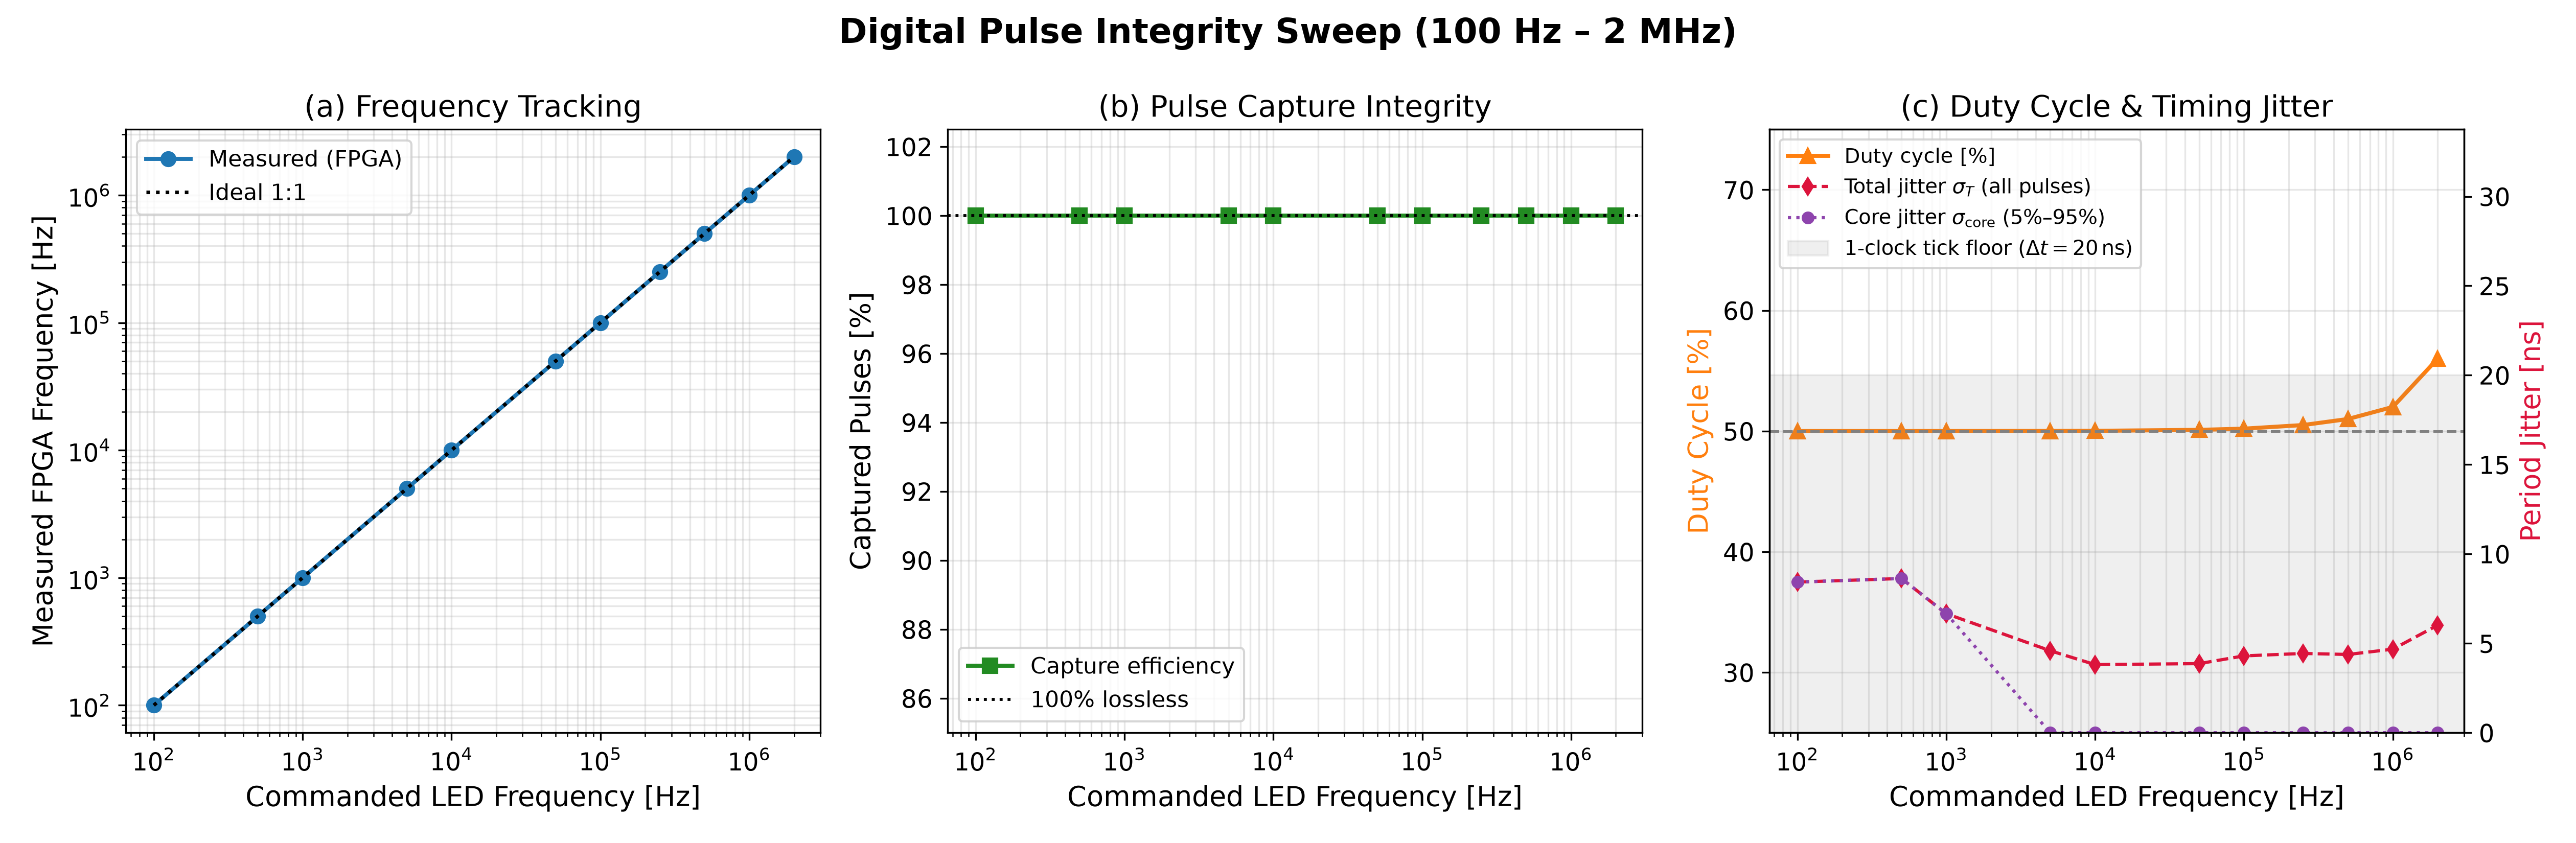
\includegraphics[width=\textwidth]{images/led_bandwidth_calibration.png}
    \caption{Digital pulse integrity validation of the FPGA DAQ ($f_s = 50\text{ MHz}$) using a pulsed red LED from $100\text{ Hz}$ to $2\text{ MHz}$: (a) frequency tracking; (b) pulse capture; (c) duty cycle stability and sub-clock period jitter.}
    \label{fig:led_pwm_sweep}
\end{figure}

\subsection{Analysis of Metrics}
The data presented in \cref{tab:led_pwm_results} and \cref{fig:led_pwm_sweep} demonstrate:
\begin{itemize}
    \item \textbf{Lossless Capture and 1:1 Frequency Tracking:} The measured frequency $f_{\text{meas}}$ matches the commanded frequency $f_{\text{set}}$ across all eleven tested steps (\cref{fig:led_pwm_sweep} a). Furthermore, the receiver captured all the pulses with zero missed events throughout the entire $100\text{ Hz}\text{--}2\text{ MHz}$ range (\cref{fig:led_pwm_sweep} b).
    
    \item \textbf{Duty Cycle Stability and Optical Turn-Off Response:} From $100\text{ Hz}$ to $10\text{ kHz}$, the digitized signal maintains an almost ideal symmetric square wave ($50.00\%\text{--}50.02\%$). As the operating frequency increases beyond $50\text{ kHz}$, the duty cycle widens gradually to $50.50\%$ at $250\text{ kHz}$ and reaches $56.00\%$ at $2\text{ MHz}$ (\cref{fig:led_pwm_sweep} c and \cref{tab:led_pwm_results}). This minor duty-cycle stretching is physical: standard LEDs exhibit a turn-off decay slightly slower than the fast electrical turn-on edge. At microsecond periods ($T = 500\text{ ns}$ at $2\text{ MHz}$), this tail remains above the comparator threshold $V_{\text{TH}}$ for an additional $\sim 30\text{ ns}$ ($\sim 6\%$ of the cycle), slightly extending the high state without causing pulse dropouts.
    
    \item \textbf{Sub-Clock Period Jitter ($\sigma_T$):} At $f_s = 50\text{ MHz}$ ($\Delta t = 20\text{ ns}$), the theoretical digital quantization floor governing a uniform-sampling edge detector is \cite[Chap 4.]{widrowQuantizationNoiseRoundoff2008}:
    \begin{equation}
        \sigma_{\text{quant}} = \frac{\Delta t}{\sqrt{6}} = \frac{20\text{ ns}}{\sqrt{6}} \approx 8.16\text{ ns}
    \end{equation}
    Across all eleven frequency steps, the measured period jitter $\sigma_T$ remains strictly bounded between $3.8\text{ ns}$ and $8.6\text{ ns}$ (\cref{fig:led_pwm_sweep} c), remaining below the single-clock period floor ($\Delta t = 20\text{ ns}$) and closely matching the theoretical quantization limit. This verifies that the BPW34 photodiode and TLV3542 Schmitt trigger (\cref{sec:circuit_schematic}) introduce negligible analog transition noise, confirming that the digital timing precision is primarily governed by the FPGA sampling clock.
\end{itemize}

\subsection{FPGA vs. Microcontroller (ESP32) for High-Speed Data Acquisition}
Although a low-cost microcontroller such as the ESP32 is well suited for generating test PWM signals and driving stepper motors, delegating high-speed pulse acquisition to the FPGA provides fundamental architectural advantages:
\begin{itemize}
    \item \textbf{Deterministic Hardware Parallelism vs.\ Interrupt Jitter:} On the FPGA, input synchronization, edge detection, and Block RAM packing execute concurrently in dedicated logic on every $20\text{ ns}$ clock cycle with zero interrupt latency. By contrast, an ESP32 relies on CPU execution shared with FreeRTOS scheduler ticks, flash-cache misses, and serial background routines. Attempting software-based GPIO sampling at megahertz rates inevitably results in non-deterministic latency and dropped edges.
    \item \textbf{Lossless Timestamping vs.\ Peripheral Bottlenecks:} While the ESP32 includes a hardware Pulse Counter (\texttt{PCNT}) capable of counting edges up to $40\text{ MHz}$, it functions only as an accumulator register: it cannot record individual edge timestamps or reconstruct instantaneous velocity profiles $v(t)$, duty cycles, or period jitter. Continuous DMA capture via the ESP32 \texttt{I2S} parallel peripheral is limited internal SRAM ($\sim 320\text{ KB}$, sustaining only milliseconds of raw data) and exhibits sample-skipping near $20\text{ MHz}$. In contrast, the Arty Z7-20, integrated with the ICTP ComBlock and PYNQ \cref{sec:comblock_API}, sustains continuous lossless $50\text{ MHz}$ acquisition buffered through FPGA BRAM into $512\text{ MB}$ of external DDR3 memory.
\end{itemize}


